\section{Konzeption}

In diesem Kapitel werden die Anforderungsdefinitionen des Projektes, mit Spezialisierung auf die verschiedenen Use Cases beschrieben.

\subsection{Anforderunsdefinitionen}
%Was wollen wir von der SOftware haben
In diesem Abschnitt wird auf die Funktionalitäten und Use Cases des Projektes eingegangen.

\subsubsection{Softwarearchitektur}
\subsection{Szenarios}
\subsection{Use Cases}
\subsubsection{Connect}

\begin{figure}[h]
	\begin{center}
		\includegraphics[width=0.8\textwidth]{images/use_cases/Connect.png}
	\end{center}
	\caption{Connect}
	\label{fig:UC_Connect}
\end{figure}

\noindent
Im Use Case Connect wird eine erste Verbindung durch die Eingabe der IP-Adresse zum Backend aufgebaut. Dabei sendet die Komponente, ob Roboter oder App eine Abbildung seiner selbst als Objekt dem Backend. Daraufhin startet das Backend die Verbindung indem es der Komponente entsprechende Verbindungskommandos zusendet. Sobald eine Reaktion in einer festgelegten Zeit erfolgt, akzeptiert das Backend die Verbindung und sendet die entsprechende Id für die Komponente. Ab diesem Moment ist die Komponente verbunden und ein Robot für Aktionen entsprechend verfügbar. Die Verbindungsinitialisierung dient hierbei der Verkürzung der Reaktionszeit, die bei einem Roboter sonst entsprechend hoch wäre.

\begin{figure}[!tbp]
	\centering
	\subfloat[Connect]{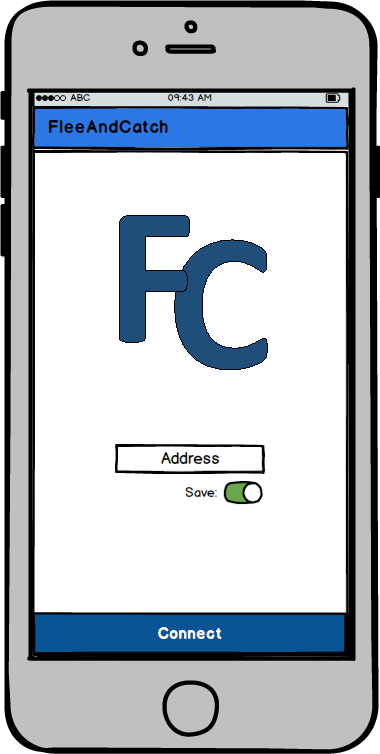
\includegraphics[width=0.4\textwidth]{images/mockups/Connection.png}\label{fig:Connect}}
	\hfill
	\subfloat[Home]{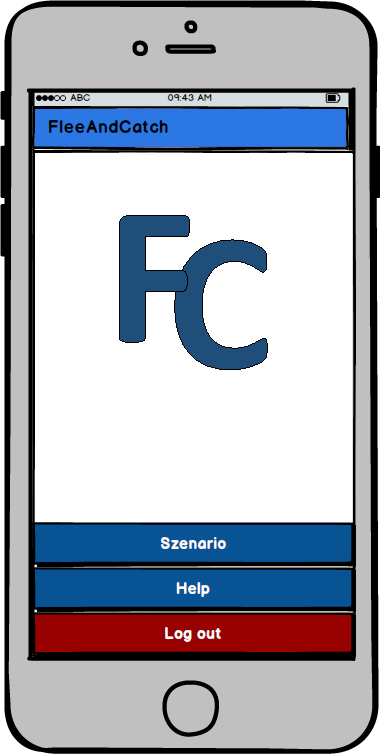
\includegraphics[width=0.4\textwidth]{images/mockups/Home.png}\label{fig:Home}}
	\caption{Connection}
\end{figure}

\subsubsection{Synchronization}

\begin{figure}[!tbp]
	\centering
	\subfloat[Update all]{\includegraphics[width=0.4\textwidth]{images/use_cases/Synchronization.png}\label{fig:UC_Synchronization}}
	\hfill
	\subfloat[Update]{\includegraphics[width=0.55\textwidth]{images/use_cases/Update.png}\label{fig:UC_Update}}
	\caption{Synchronization}
\end{figure}

\noindent
Im Use Case Synchronization werden Daten entsprechend des gesetzten Typen zwischen den Komponenten übertragen. Dabei können einerseits die Roboter als Objekte, oder ganze Szenarien übertragen werden. Dies dient zur Gegenseitigen Synchronisierung der Daten.

\begin{figure}[!tbp]
	\begin{center}
		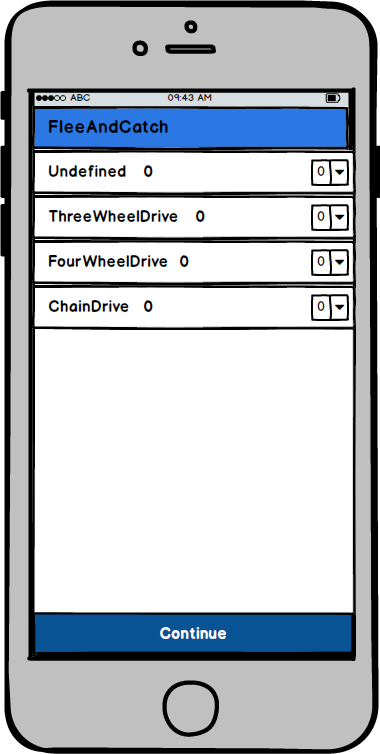
\includegraphics[width=0.5\textwidth]{images/mockups/RobotList.png}
	\end{center}
	\caption{Robot list}
	\label{fig:RobotList}
\end{figure}

\subsubsection{Szenario}

\begin{figure}[h]
	\begin{center}
		\includegraphics[width=0.6\textwidth]{images/use_cases/Spectator.png}
	\end{center}
	\caption{Spectator}
	\label{fig:UC_Spectator}
\end{figure}
\begin{figure}[h]
	\begin{center}
		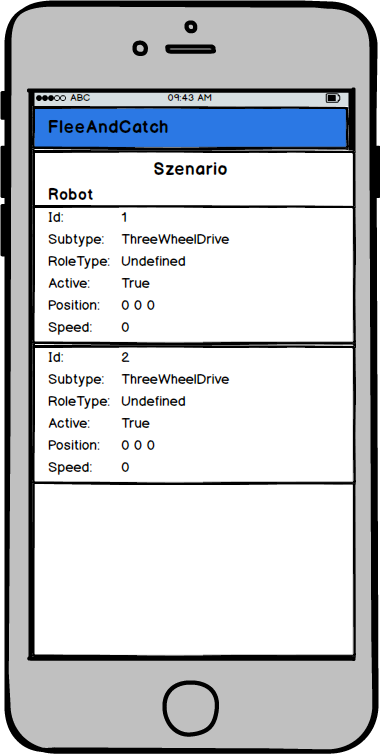
\includegraphics[width=0.6\textwidth]{images/mockups/Spectator.png}
	\end{center}
	\caption{Spectator}
	\label{fig:Spectator}
\end{figure}

\begin{figure}[h]
	\begin{center}
		\includegraphics[width=0.8\textwidth]{images/use_cases/Control.png}
	\end{center}
	\caption{Control}
	\label{fig:UC_Control}
\end{figure}
\begin{figure}[h]
	\begin{center}
		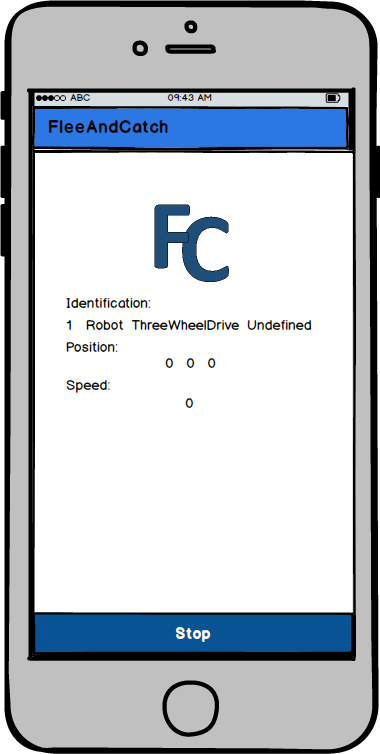
\includegraphics[width=0.6\textwidth]{images/mockups/Control.png}
	\end{center}
	\caption{Control}
	\label{fig:Control}
\end{figure}

\begin{figure}[h]
	\begin{center}
		\includegraphics[width=0.9\textwidth]{images/use_cases/Synchron.png}
	\end{center}
	\caption{Synchron}
	\label{fig:UC_Synchron}
\end{figure}

\begin{figure}[h]
	\begin{center}
		\includegraphics[width=0.9\textwidth]{images/use_cases/Follow.png}
	\end{center}
	\caption{Follow}
	\label{fig:UC_Follow}
\end{figure}

\subsubsection{Exception}
\subsection{Kommunikation}